% !TeX root = ../index.tex
\documentclass[../index.tex]{subfiles}
\begin{document}
    \section{Wykład}
        Gwiazdy kończą swoję życie jako białe karły, gwiazdy neutronowe lub czarne dziury w większości w zależności od masy:
        \begin{itemize}
            \item do 9-10 mas Słońca \( \to \) biały karzeł
            \item od 10 do 25-40 mas Słońca \(\to \) gwiazda neutronowa
            \item od 25-40 mas Słońca \(\to \) czarna dziura
        \end{itemize}
        \subsection{Białe karły}
            Białe karły zbudowane są z bardzo gęsto upakowanej masy, np. Syriusz B ma rozmiary Ziemi i masę słońca. Wykazują one zależność masy i promienia (\(M\sim R^{ - \frac{1}{3}}\)) oraz istnieje pewna maksymalna masa białego karła, powyżej której zapada się on grawitacyjnie do gwiazdy neutronowej. Wielkość ta nosi nazwę \textbf{masy Chandrasekhara}:
            \begin{equation}
                M_\text{Ch} =\autoround{\frac{5.75}{\mu_e^2}}M_\odot
            \end{equation}
            Dla \(\mu_e = 2\)(ciężar cząsteczkowy w przeliczeniu na jeden elektron) otrzymuje się wynik \(M_\text{Ch} = 1.44M_\odot\). Zbudowane są one ze zdegenerowanej materii i otaczjącej jej cienkiej warstwy zwykłego gazu. Białe karły charakteryzuje niska moc promieniowania. Białe karły można klasyfikować na podstawie ich widma:
            \begin{itemize}
                \item DA – tylko linie balmera
                \item DB – tylko linie He I
                \item DC – żadnych linii
                \item DO – wyróżnia się linie He II
                \item DZ – tylko linie metali
                \item DQ – wyróżnia się linie węgla
            \end{itemize}
            Linie tych widm są bardzo szerokie, co wskazuje na wysokie wartości ciśnienia. Najwięcej jest biały karłów w przedziale mas \(0.5 - 0.8 M_\odot\), a ich temperatura jest raczej niższa niż \(7000\:K\)/. Białe karły święcą kosztem swojej energii wewnętrznej w wyniku czego stygną. W miarę tego procesu materia we wnętrzu karła zaczyna wykazywać cechy najpierw cieczy, a później ciała stałego – następuje krystalizacja. Moc promieniowania także się zmienia – maleje wraz ze stygnięciem. Mierząc liczność białych karłów o różnej mocy promieniowania  można mierzyć wiek gromad gwiazd. Im więcej słabo świecących karłów tym starsza.
        \subsection{Gwiazdy neutronowe}
            Nie wiemy dokładnie jak zbudowane są gwiazdy neutronowe – wciąż trwają prace nad modelami, które będą jednocześnie dobrze odzwierciedlały dane obserwacyjne jak i wykorzystywały wiedzę na temat egzotycznych stanów materii. Można mówić o dwóch klasach modeli \textbf{minimalnych} i \textbf{egzotycznych}. W obu przypadkach wyróżnia się \textbf{skorupę}, \textbf{płaszcz} i \textbf{jądro}, a głównym składnikiem gwiazdy jest zdegenerowana ciecz neutronowa wykazująca cechy nadciekłości.
            \begin{itemize}
                \item model minimalny:
                \begin{center}
                    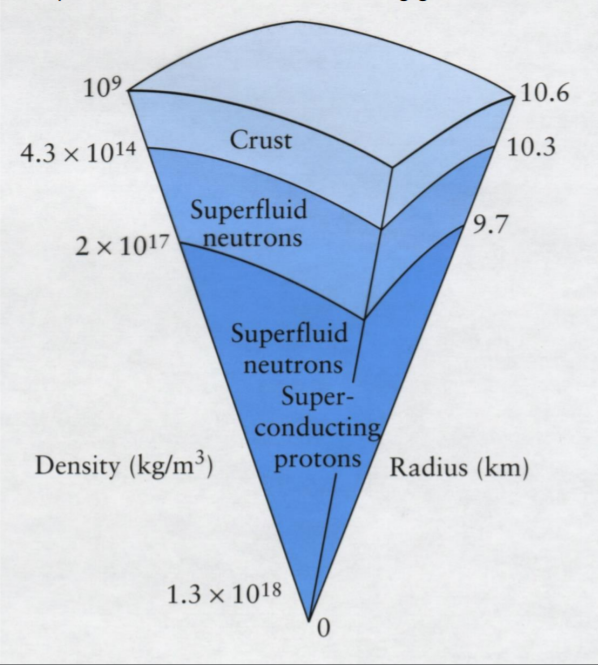
\includegraphics[width=11cm]{images/gwiazdaNeutronowaModelMinimalny.png}
                \end{center}
                \item model egzotyczny:
                \begin{center}
                    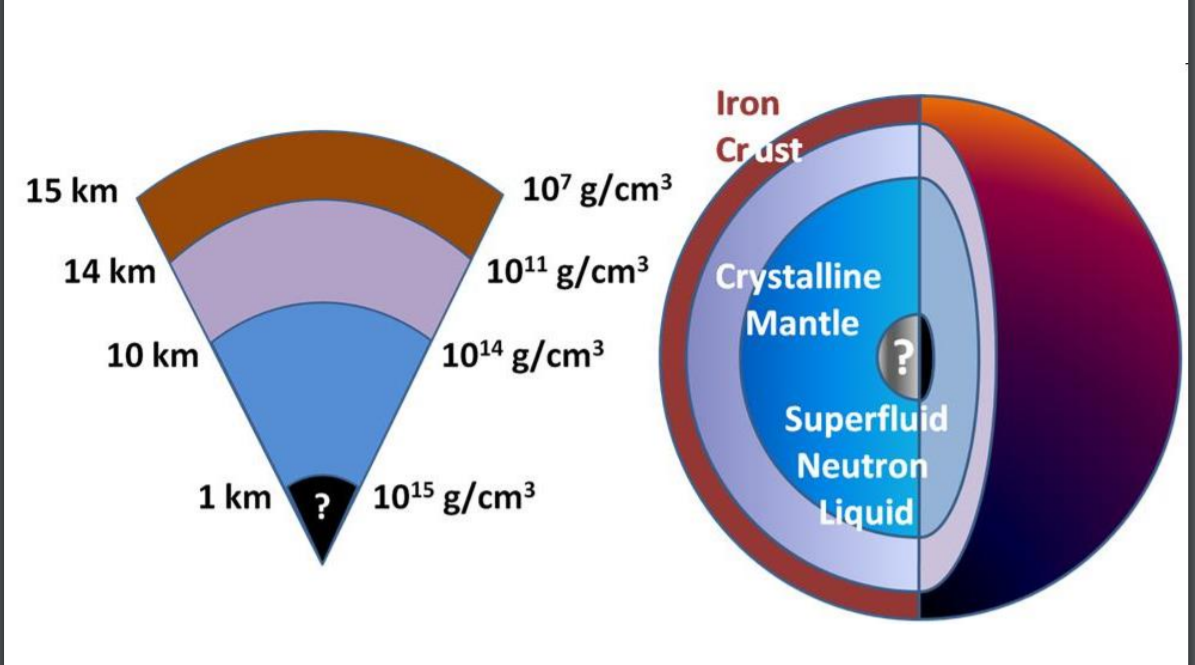
\includegraphics[width=15cm]{images/gwiazdaNeutronowaModelEgzotyczny.png}
                \end{center}
            \end{itemize}
            Podobnie jak białe karły wykazują zależność promień-masa, a po przekroczeniu maksymalnej masy – \textbf{masy Tolmana–Oppenheimera-Volkoffa} następuje kolaps do czarnej dziury. Różne model podają różne masy krytyczne. Większość modeli pokazuje, że gwiazdy neutronowe nie przekraczają dwóch mas słońca, ale pojedyncze obserwacje sugerują istnienie takich osiągających trzy masy słońca i dopiero tą wartość uznaje się za próg mas gwiazd neutronowych. Gwiazdy neutronowe także stopniowo stygną emitując promieniowania kosztem energii wewnętrznej. Ze względu na bardzo niewielkie rozmiary (rzędu kilkunastu kilometrów) rotacja gwiazd neutronowych może osiągać zawrotne prędkości. Dodatkowo wytwarzają one silne pola magnetyczne. Te dwie cechy powodują, że cząstki naładowane uwięzione w ich polu elektryczny emitują \textbf{promieniowanie synchrotronowe} – najsilniejsze w okolicach biegunów magnetycznych – gwiazda jest \textbf{pulsarem}. Pulsar to obiekt astronomiczny emitujący regularne nietermiczne impulsy elektromagnetyczne (\textbf{pulsar milisekundowy} to taki pulsar, w którym odstępy pomiędzy kolejnym impulsami są rzędu milisekund, a czas trwania impulsu jest długi w porównaniu do tej przerwy).
            \begin{center}
                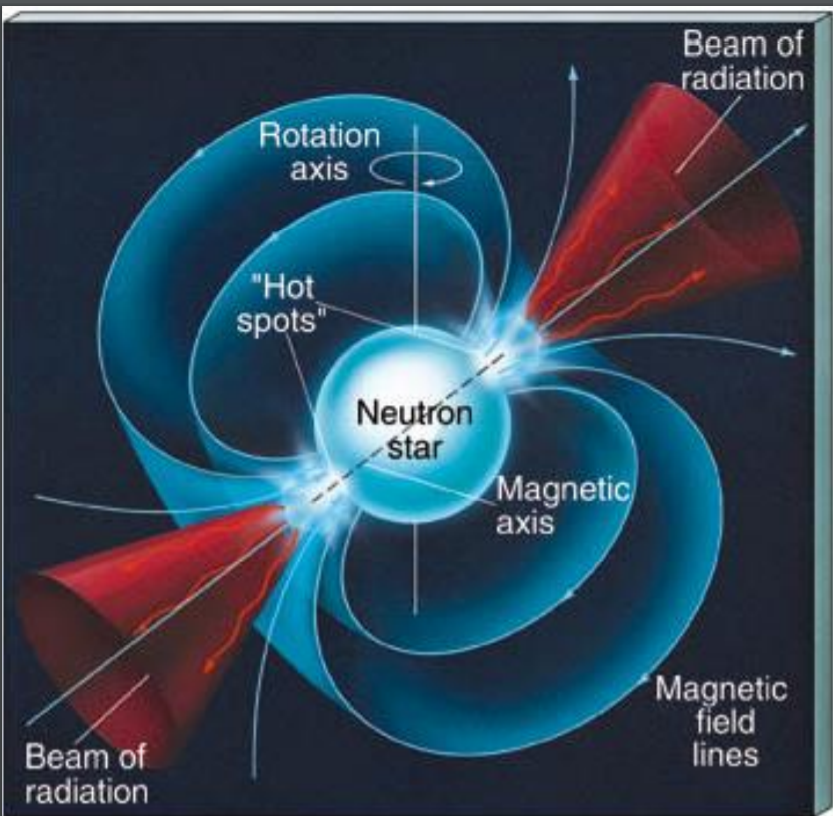
\includegraphics[width=13cm]{images/pulsar.png}
            \end{center}
            W skutek powolnego wytracania momentu pędu przez pulsar, jego okres się wydłuża. Nie obserwuje się pulsarów o okresach dłuższych o kilka sekund (gwiazdy neutronowe tak stare, że ich okres miałby taką wartość przestają efektywnie produkować promieniowania synchrotronowe).
        \subsection{Czarne dziury}
            Powstają w wyniku kolapsu gwiazdy do jednego punktu – \textbf{osobliwości}. Osobliwości nie można dostrzec bezpośrednio, ponieważ otacza ją przestrzenie ograniczona \textbf{horyzontem zdarzeń} – obszar z którego druga prędkość kosmiczna (prędkość ucieczki) jest większa niż prędkość światła – na zewnątrz nie może wydostać się żadna informacja. W modelu nierotującej \textbf{czarnej dziur Schwarzschilda} promień horyzontu zdarzeń jest równy \textbf{promieniowi Schwarzschilda}:
            \begin{equation}
                r_s = \frac{2 G M}{c^2 } 
            \end{equation}
            W przypadku rotującej czarnej dziury stosuje się model \textbf{czarnej dziury Kerra}. Ta posiada dwa horyzonty zdarzeń – jeden wewnętrzny i sferyczny oraz drugi – zewnętrzny i elipsoidalny. Strefa pomiędzy nimi nosi nazwę \textbf{egzosfery} i może z niej wydostawać się promieniowanie, ale jest zmuszona do rotowania razem z czarną dziurą. Czarną dziurę można zaobserwować na jeden z trzech sposobów:
            \begin{itemize}
                \item w wyniku ugięcia czasoprzestrzeni czarna dziura może działać jak soczewka 
                \item poprzez detekcje fal grawitacyjnych wywołanych zjawiskiem połączenia się dwóch czarnych dziur
                \item obserwacje akrecji materii (opadania materii) na czarną dziurę (dotyczy układów podwójnych).
            \end{itemize}
\end{document}